\section{Durchführung}
\label{sec:Durchführung}

Der Aufbau des Michelson-Interferometers ist in Abbildung \ref{fig:bild1} dargestellt.
Die Apparatur muss so justiert werden, dass die Überschneidung der beiden hellsten Punkte detektiert wird.

\begin{figure}
    \centering
    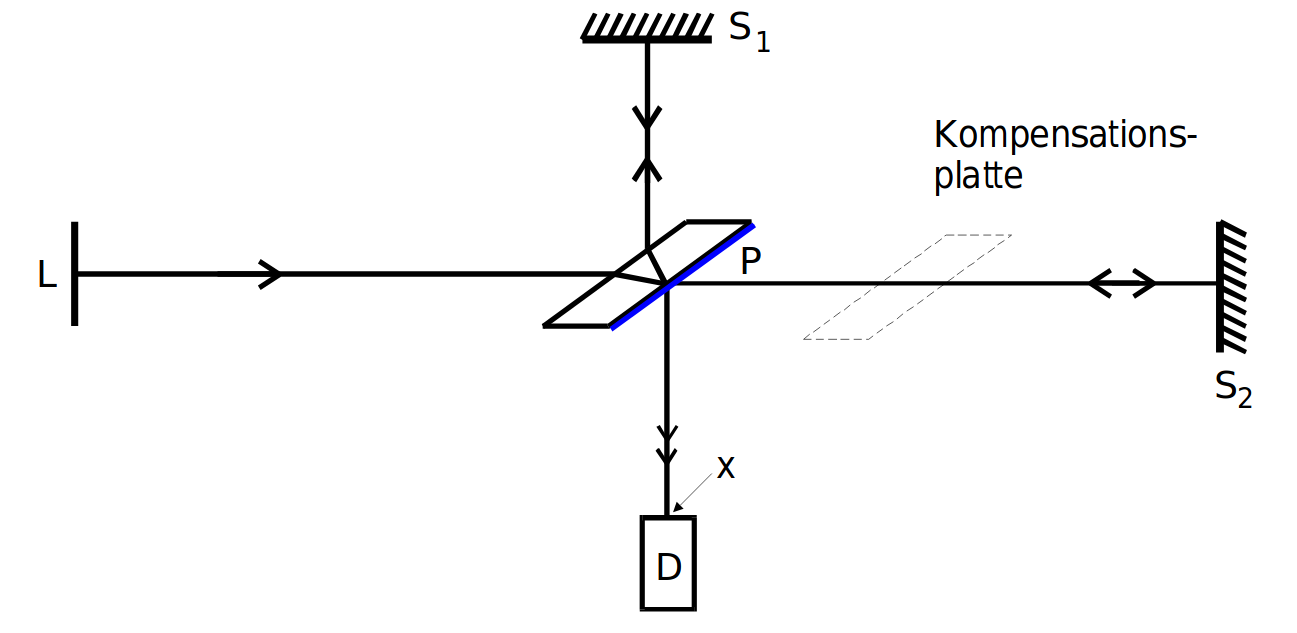
\includegraphics[scale = 0.2]{content/bild1.png}
    \caption{Prinzipieller Aufbau des Michelson-Interferometers.
            Das Licht wird von der Lichtquelle $L$ emittiert, trifft auf den Strahlenteiler $P$, das reflektierte
            Lichtbündel trifft auf den Spiegel $S_1$, das transmittierte auf $S_2$. Danach treffen sie wieder auf 
            $P$ und jeweils ein Teil trifft auf den Detektor $D$ und interferiert dort mit dem anderen. [1]}
    \label{fig:bild1}
  \end{figure}

Damit die beiden Lichtbündel kohärent zueinander bleiben, muss ihr optischer Wegunterschied kleiner als
die Kohärenzlänge 

\begin{equation}
  l = n \lambda
\end{equation}

der Lichtquelle sein. Dabei ist $n$ die Anzahl der bei $D$ beobachtbaren Intensitätsmaxima. 
Die Bedingung wird dadurch realisiert, dass für die Abstände

\begin{equation}
    \overline{S_1 P} \approx \overline{S_2 P}
    \label{eqn:approx}
\end{equation}

gilt. Zudem wird zwischen $P$ und $S_2$ eine Kompensationsplatte eingebaut. Diese gleicht, dass das reflektierte
Lichtbündel die Spiegelplatte von $P$ zweimal mehr durchläuft, als das transmittierte.

Trifft \eqref{eqn:approx} genau zu, so kommt es am Detektor zur destruktiven Interferenz.


Mit einem hoch untersetzten Zahnradmotor wird die Mikrometerschraube des Spiegels $S_1$ gedreht und dieser
um $\symup{\Delta} d$ verschoben. Es werden $z = 3000$ von den auftretenden Interferenzringen gemessen.

Außerdem gilt: 
\begin{equation}
    \frac{\symup{\Delta}d}{C_\text{H}} = \frac{z \cdot \lambda}{2}
    \label{eqn:eins}
\end{equation}

mit dem Hebelübersetzungsfaktor $C_\text{H}$.

Für die Messung des Brechungsindizes $n$ wird die in Abbildung \ref{fig:bild2} abgebildete
Versuchsanordnung werwendet.

\begin{figure}
    \centering
    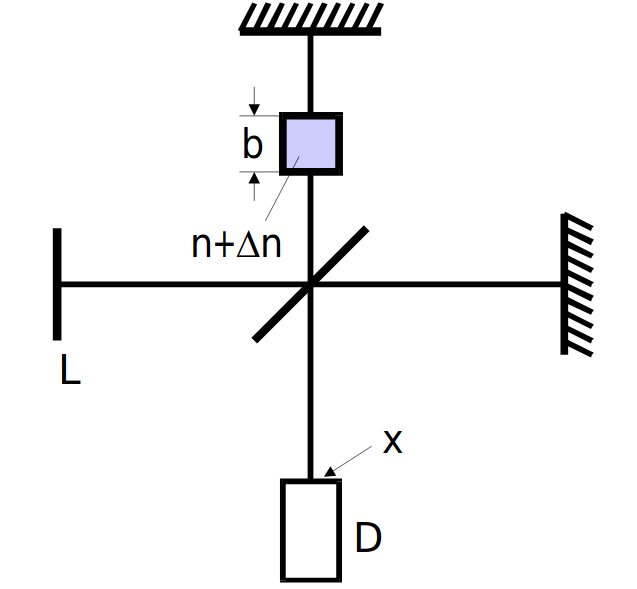
\includegraphics[scale = 0.2]{content/bild2.png}
    \caption{Aufbau des Michelson-Interferometers mit einem Abschnitt der Länge $b$ und des
    Brechungsindizes $n + \symup{\Delta}n$ zwischen $P$ und $S_1$ [1]}
    \label{fig:bild2}
  \end{figure}

  Der Wegunterschied zwischen den Strahlenbündeln beträgt dann $\symup{\Delta}nb$ und
  kann durch Senkung des Luftdruckes in der Messzelle vergrößert werden. Es gilt dann:

  \begin{equation}
    \symup{\Delta}nb = \frac{z \cdot \lambda}{2}
    \label{eqn:delta}
  \end{equation}

  und $n$ ergibt sich zu

  \begin{equation}
      n(p_0, T_0) = 1 + \symup{\Delta} n (p,p') \frac{T}{T_0} \frac{p_0}{p - p'} \; .
      \label{eqn:brech}
  \end{equation}


